Kolejnym rozkładem, który koniecznie musimy poznać jest rozkład normalny - rozkład Gaussa. \\

\begin{definition}
    Rozkład normalny oznaczamy \(N(\mu , \sigma^2 )\).\\
    \(\mu\) - wartość oczekiwana,
    \(\sigma^2\) - wariancja
\end{definition}

\begin{definition}
    Standardowy rozkład Normalny oznaczamy \(N(0, 1)\).
\end{definition}

Rozkład normalny można zobaczyć w wynikach kolosów niektórych przedmiotów (na pewno nie z MD)

\begin{definition}
    Funkcja gęstości rozkładu normalnego wynosi: \[ f_Z(z) =  \frac{1}{\sigma\sqrt{2\pi}}e^{-((z - \mu)/\sigma)^2/2} \]
    Dla standardowego rozkładu normalnego:
    \[ \phi(z) =  \frac{1}{\sqrt{2\pi}}e^{-z^2/2} \]
\end{definition}

Standardowy rozkład normalny wygląda jak \sout{dzban} dzwon.

\begin{figure}[H]
    \centering
    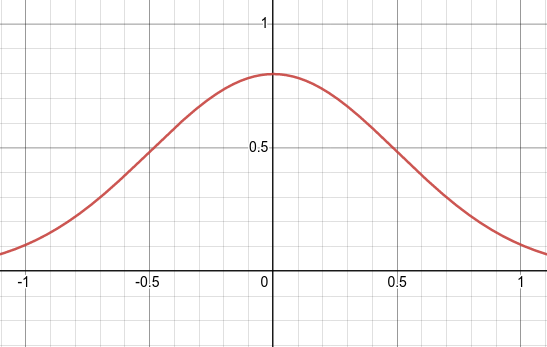
\includegraphics[scale=0.75]{img/normal-distribution/normal-distribution-0-0.5.png}
    \caption{Rozkład normalny z parametrami \( \mu = 0, \sigma = 0.5 \)}
\end{figure}

\begin{definition}
    Dystrybuanta to oczywiście całka gęstości:
    \[
    F_Z(z) = \frac{1}{\sqrt{2\pi}\sigma}\int_{-\infty}^{z}e^{-((t -\mu)/\sigma)^2/2} dt
    \]
    Oraz dla standardowego:
    \[
    \Phi(z) = \frac{1}{\sqrt{2\pi}}\int_{-\infty}^{z}e^{-t^2/2} dt
    \]
\end{definition}

Policzenie tej całki jest niemożliwe metodą analityczną więc w celu wyliczenia danej wartości stosuje się tablice dla standardowego rozkładu normalnego. 
